\documentclass[a4paper]{article}

% Packages
\usepackage{amsmath}
\usepackage{amssymb}
\usepackage{amsthm}
\usepackage{bold-extra}
\usepackage{fancyhdr}
\usepackage{geometry}
\usepackage{graphicx}
\usepackage{hyperref}
\usepackage{ifthen}
\usepackage[utf8]{inputenc}
\usepackage{multirow}
\usepackage{needspace}
\usepackage{parskip}
\usepackage{stmaryrd}
\usepackage{listings}
\usepackage[T1]{fontenc}
\usepackage{longtable}
\usepackage{comment}
\usepackage{enumerate}
\usepackage{xspace}
\usepackage{textcomp}
\usepackage{array}

\usepackage{tikz}
\usetikzlibrary{automata,positioning,shapes.geometric}
\usepackage{tikzsymbols}
\usepackage{todonotes}

\lstset{language=Java, numbers=left, showstringspaces=false, tabsize=4}
\geometry{a4paper, left=25mm,right=25mm, top=25mm, bottom=25mm}

% check for the existence of commands
\newcommand{\checkfor}[3]{%
  \ifcsname#1\endcsname%
  #2
  \else%
  #3
  \fi%
}

\checkfor{exnumber}{}{\newcommand{\exnumber}{-1}}

\newcommand{\exercisepagebreak}{\checkfor{isexercise}{\pagebreak}{}}
\newcommand{\solutionpagebreak}{\checkfor{isexercise}{}{\pagebreak}}

\setcounter{section}{\exnumber{}}

\numberwithin{equation}{section}
\numberwithin{figure}{section}
\numberwithin{table}{section}
\renewcommand{\qedsymbol}{\textsc{q.e.d.}}
\renewenvironment{proof}[1][\proofname]{{\bfseries #1: }}{\qed}
\newtheoremstyle{defstyle}{10pt}{5pt}{\addtolength{\leftskip}{2\leftmargini}\addtolength{\rightskip}{2\leftmargini}}{-1\leftmargini}{\scshape\bfseries}{:}{\newline}{#1 #2\ifthenelse {\equal {#3}{}} {}{ (\text{\textsc{#3}})}}{}
\newtheoremstyle{thmstyle}{10pt}{5pt}{\addtolength{\leftskip}{2\leftmargini}\addtolength{\rightskip}{2\leftmargini} \slshape}{-1\leftmargini}{\scshape\bfseries}{:}{\newline}{#1 #2\ifthenelse {\equal {#3}{}} {}{ (\text{\textsc{#3}})}}{}
\newtheoremstyle{exstyle}{10pt}{5pt}{\addtolength{\leftskip}{2\leftmargini}\addtolength{\rightskip}{2\leftmargini}}{-1\leftmargini}{\scshape\bfseries}{:}{\newline}{#1 #2\ifthenelse {\equal {#3}{}} {}{ (\text{\textsc{#3}})}}{}
\newtheoremstyle{algostyle}{10pt}{5pt}{\addtolength{\leftskip}{2\leftmargini}\addtolength{\rightskip}{2\leftmargini}}{-1\leftmargini}{\scshape\bfseries}{:}{\newline}{#1\ifthenelse {\equal {#3}{}} { #2}{ \text{\textsc{#3}}}}{}
\theoremstyle{defstyle}
\newtheorem{mydef}{Definition}[section]
\theoremstyle{thmstyle}
\newtheorem{mythm}{Theorem}[section]
\newtheorem{mylem}[mythm]{Lemma}
\newtheorem{myprop}[mythm]{Proposition}
\theoremstyle{exstyle}
\newtheorem{myex}{Example}[section]
\theoremstyle{algostyle}
\newtheorem{myalgo}{Algorithm}

% Define programming and solution environment and only use if enabled
\checkfor{isprog}{
  % Define exercise environment
  \newcounter{exercise}
  \newenvironment{exercise}[1]{\refstepcounter{exercise}\label{ex\theexercise}\section*{Programming Exercise \theexercise \hfill (#1 Points)}}{}
  \checkfor{isexercise}{
    % Programming exercise
    \excludecomment{solution}
    \excludecomment{onlysolution}
    \newenvironment{onlyexercise}{}{}
    \newcommand{\extitle}{Programming Exercise}
  }{
    % Programming solution
    \newenvironment{solution}{\label{sol\theexercise}\subsection*{Solution: \hrulefill}}{}
    \newenvironment{onlysolution}{}{}
    \excludecomment{onlyexercise}
    \newcommand{\extitle}{Programming Solution}
    }
}{
  % Define exercise environment
  \newcounter{exercise}
  \newenvironment{exercise}[1]{\refstepcounter{exercise}\label{ex\theexercise}\section*{Exercise \theexercise \hfill (#1 Points)}}{}
  \checkfor{isexercise}{
    % Theoretical exercise
    \excludecomment{solution}
    \excludecomment{onlysolution}
    \newenvironment{onlyexercise}{}{}
    \newcommand{\extitle}{Exercise Sheet}
  }{
    % Theoretical solution
    \newenvironment{solution}{\label{sol\theexercise}\subsection*{Solution: \hrulefill}}{}
    \newenvironment{onlysolution}{}{}
    \excludecomment{onlyexercise}
    \newcommand{\extitle}{Solution}
  }
}

% Define header
\pagestyle{fancy}
\fancyhf{} % Clear all headers
\setlength{\headsep}{25pt}
\cfoot{\thepage} % Page numbers
\lhead{ % Header-Definition
  % Logo
  \begin{tabular}[b]{l l}
      \multirow{2}{38mm}{
        \raisebox{-3.6mm}[0pt][0pt]{
          \includegraphics[height=14mm]{../i2}
        }
      }
      & Lehrstuhl f{\"u}r Informatik 2 \\
      & Software Modeling and Verification
    \end{tabular}
}
\rhead{ % Header-Definition
  % Course name
  \begin{tabular}[b]{r}
    Compiler Construction 2025\\
    \extitle{} \exnumber
  \end{tabular}
}
\AtBeginDocument{
  \vspace*{-30pt}
  apl.\ Prof.\ Dr.\ Thomas Noll\hfill Daniel Zilken, Roy Hermanns
  \vspace{5mm}
}


\newcommand{\header}[1]{
  % Header
  \begin{center}
    {\huge \textbf{Compiler Construction 2025}}\\
    \vspace*{1\baselineskip}%
    {\huge \textbf{--- \extitle{} \exnumber{} ---}}\\
    \checkfor{isexercise}{
      \vspace*{1\baselineskip}
      \checkfor{isprog}{
        %Upload in Moodle until #1 before the exercise class.
      }{
        Upload in Moodle or hand in until #1 before the exercise class.
      }
    }{}
    \vspace*{1.5\baselineskip}
    \hrule
  \end{center}
}

% Change numbering to (a) and (i)
\renewcommand{\labelenumi}{(\alph{enumi})}
\renewcommand{\labelenumii}{(\roman{enumii})}

% Custom commands
\newcommand{\TODO}[1]{\color{red}\textbf{TODO:} #1\color{black}}

% Macros
\newcommand{\set}[1]{\ensuremath{\left\{ #1 \right\}}}
\newcommand{\Nats}{\ensuremath{\mathbb{N}}}
\newcommand{\Reals}{\ensuremath{\mathbb{R}}}

\newcommand{\PTIME}{\mbox{\rm PTIME}}
\newcommand{\PSPACE}{\mbox{\rm PSPACE}}
\newcommand{\coNP}{\mbox{\rm coNP}}
\newcommand{\NP}{\mbox{\rm NP}}
\newcommand{\poly}{\mbox{\rm poly}}
\newcommand{\coPTIME}{\mbox{\rm coPTIME}}
\newcommand{\coPSPACE}{\mbox{\rm coPSPACE}}
\newcommand{\NPSPACE}{\mbox{\rm NPSPACE}}
\def\EXPTIME{\text{\rm EXPTIME}}
\def\doubleEXPTIME{\text{\rm 2EXPTIME}}

% Lecture specific commands
\renewcommand{\L}{{\cal L}}
\newcommand{\numberone}{\ensuremath{\set{1, \dots, 9}}}
\newcommand{\numberzero}{\ensuremath{\set{0, \dots, 9}}}
\newcommand{\eps}{\ensuremath{\varepsilon}}
\newcommand{\sem}[1]{\llbracket#1\rrbracket}
\newcommand{\la}{\ensuremath{\textsf{la}}}
\newcommand{\fir}{\ensuremath{\textsf{fi}}}
\newcommand{\first}{\ensuremath{\textsf{first}}}
\newcommand{\fo}{\ensuremath{\textsf{fo}}}
\newcommand{\follow}{\ensuremath{\textsf{follow}}}
\newcommand{\cyl}[1]{\ensuremath{\mathit{Cyl}(#1)}}
\newcommand{\icompiler}[0]{\texttt{i2Compiler}}
\newcommand{\while}[0]{\textit{WHILE}\xspace}



\begin{document}

\header{November 9th}

\begin{onlysolution}
  \begin{center}
    \includegraphics[scale=1.0]{xkcd_leftpar}

    \scriptsize Credit: \href{https://xkcd.com/859/}{https://xkcd.com/859/}
  \end{center}
\end{onlysolution}

%\section*{General Remarks}
%\begin{itemize}
  %
  %\item If you have questions regarding the exercises, feel free to write us an email at \href{mailto:cc22@i2.informatik.rwth-aachen.de}{cc22@i2.informatik.rwth-aachen.de}.
  %
  %
  %\item Exercises are \emph{optional}, i.e., not required for admission to exams. However, corrections to students’ solutions are provided as annotations to the submissions.
  %
  %\item You can hand in your solution to the tasks digitaly in the Moodle room. Alternatively, you can hand in your solution to the tasks at our chair in the corresponding box or before the exercise class.
  %
  %\item Please hand in your solutions in \emph{groups of four} and hand in only one solution per group. You can use the forum in this Moodle room to find group members.
%\end{itemize}

\begin{exercise}{15+10+10}
\begin{enumerate}
  \item[(a)] In order to design a lexer for our Java-style programming language \while, we want to define a mapping from lexemes to symbols. Complete the following table where we already defined the lexemes and the symbol class for identifiers. Assign to each lexeme in the table an appropriate symbol class, token, and symbol. Within a symbol, the value of a lexeme can be accessed via \emph{value}. For instance, if the lexeme \emph{abc} is an identifier, then (id, \emph{abc}) is the corresponding symbol. We use the characters \textvisiblespace{} for whitespaces, \textbackslash{}t for tabular, and \textbackslash{}n and \textbackslash{}r for newlines. Other lexemes may be expressed as regular expressions or are abbreviated with $\ldots$ to increase readability.
\newcolumntype{L}{>{\ttfamily}l}
\begin{longtable}{L|l|l|l}
      \hline
      lexeme              & symbol class ~~ & token ~~~~ & symbol ~~~~ \\
      \hline
      int        &   &  &  \\
      while      &   &  &  \\
      if         &   &  &  \\
      else       &   &  &  \\

      ==         &   &  &  \\
      <          &   &  &  \\

      !          &  &  &  \\
      \&\&       &  &  &  \\
      ||         &  &  &  \\

      +          &  &  &  \\
      *          &  &  &  \\
      /          &  &  &  \\
      \%         &  &  &  \\

      ;          &  &  &  \\
      =          &  &  &  \\
      (          &  &  &  \\
      )          &  &  &  \\
      \{         &  &  &  \\
      \}         &  &  &  \\

      0 $\mid ($- $\mid \varepsilon)\{$1$,\ldots,$9$\}\{$0$,\ldots$,9$\}^\ast$ &  &  &  \\
      $\{$a,$\ldots$,z,A,$\ldots$,Z,\_$\}\{$a,$\ldots$,z,A,$\ldots$,Z,0,$\ldots$,9,\_$\}^\ast$ & identifier & id  & (id, \emph{value}) \\
      "$\{$a,$\ldots$,z,A,$\ldots$,Z,0,$\ldots$,9,\_\textvisiblespace+-*$\ldots\}^\ast$" &  &  &  \\
      true       &  &  &  \\
      false      &  &  &  \\

      //\textnormal{\ldots (}\textbackslash{}n $\mid$ \textbackslash{}r $\mid$ \textbackslash{}r\textbackslash{}n) &  &  &  \\
      /*\textnormal{\ldots}*/     &  &  &  \\
      \textvisiblespace  &  &  &  \\
      \textbackslash{}t  &  &  &  \\
      \textbackslash{}n  &  &  &  \\
      \textbackslash{}r  &  &  &  \\

      \hline
\end{longtable}



  \item[(b)] Decompose the following program (also attached as a txt file) into a sequence of lexemes and translate each lexeme into a symbol according to your solution in \textbf{(a)}.
  
  \begin{center}
  \begin{tabular}{c}
    \begin{lstlisting}
/* collatz problem */
int n = 25;
while ( 0 < n ) {
	if (n % 2 == 0) { //even?
		n =n/2;
	} else {
		n =n*3+1;
	}
}
    \end{lstlisting}
  \end{tabular}
\end{center}

 \item[(c)] Consider the following program:
 
\begin{center}
	\begin{tabular}{c}
		\begin{lstlisting}
int intx = 25;
		\end{lstlisting}
	\end{tabular}~~~~~~~~~~~~~~~~~~~~~~~~~~~~
\end{center}
%
%
Give the sequence of symbols a lexer should produce. Give two additional (but incorrect) sequences of symbols a lexer might produce. How can the lexer ensure that the decomposition of the program into lexemes is \emph{unique}?

\end{enumerate}
\end{exercise}

\begin{solution}
\newcolumntype{L}{>{\ttfamily}l} % \texttt{} version of "l" column type

\begin{enumerate}
  \item[(a)] There are several possible ways to solve this task. For example, all keywords may be identified with the same token and distinguished only through an attribute or each keyword may be identified by a unique token. The former solution is presented here, the latter is chosen for the implementation.
\begin{longtable}{Llll}
      \hline
      lexeme              & symbol class & token & symbol \\
      \hline
      int        & keywords  & key & (key, int) \\
      while      & keywords  & key & (key, while) \\
      if         & keywords  & key & (key, if) \\
      else       & keywords  & key & (key, else) \\

      ==         & relation  & rel & (rel, eq) \\
      <          & relation  & rel & (rel, lt) \\

      !          & bool. op. & bool & (bool, not) \\
      \&\&       & bool. op. & bool & (bool, and) \\
      ||         & bool. op. & bool & (bool, or) \\

      +          & arith. op. & aop & (aop, plus) \\
      *          & arith. op. & aop & (aop, mult) \\
      /          & arith. op. & aop & (aop, divide) \\
      \%          & arith. op. & aop & (aop, mod) \\

      ;          & special symbol & sym & (sym, semicolon) \\
      =          & special symbol & sym & (sym, assignment) \\
      (          & special symbol & sym & (sym, lpar) \\
      )          & special symbol & sym & (sym, rpar) \\
      \{         & special symbol & sym & (sym, lbrace) \\
      \}         & special symbol & sym & (sym, rbrace) \\

      0 $\mid ($- $\mid \varepsilon)\{$1$\ldots$9$\}\{$0$\ldots$9$\}^\ast$ & numbers & num & (num, value) \\
      $\{$a$\ldots$zA$\ldots$Z\_$\}\{$a$\ldots$zA$\ldots$Z0$\ldots$9\_$\}^\ast$ & identifier & id & (id, value) \\
      "$\{$a$\ldots$zA$\ldots$Z0$\ldots$9\_\textvisiblespace+-*$\ldots\}^\ast$" & string constant & string & (string, value) \\
      true       & boolean constant & bconst & (bconst, true) \\
      false      & boolean constant & bconst & (bconst, false) \\

      //\textnormal{\ldots (}\textbackslash{}n $\mid$ \textbackslash{}r $\mid$ \textbackslash{}r\textbackslash{}n) & comment & cmt & (cmt, cmtsingle) \\
      /*\textnormal{\ldots}*/     & comment & cmt & (cmt, cmtmulti) \\
      \textvisiblespace  & blanks & blank & none, will be ignored \\
      \textbackslash{}t  & blanks & blank & none, will be ignored \\
      \textbackslash{}n  & blanks & blank & none, will be ignored \\
      \textbackslash{}r  & blanks & blank & none, will be ignored \\

      \hline
\end{longtable}

  \item[(b)] We have the following lexemes, where we separate lexemes by a centred dot:
    \begin{itemize}
        \item[] /* collatz problem */ $\cdot$ \textbackslash{}n
        \item[] int $\cdot$ \textvisiblespace{} $\cdot$ n $\cdot$ \textvisiblespace{} $\cdot$ = $\cdot$ \textvisiblespace{} $\cdot$ 25 $\cdot$ ; $\cdot$ \textbackslash{}n
        \item[] while $\cdot$ \textvisiblespace{} $\cdot$ ( $\cdot$ \textvisiblespace{} $\cdot$ 0 $\cdot$ \textvisiblespace{} $\cdot$ < $\cdot$ \textvisiblespace{} $\cdot$ n $\cdot$ \textvisiblespace{} $\cdot$ ) $\cdot$ \textvisiblespace{} $\cdot$ \{$\cdot$ \textbackslash{}n
        \item[] \textbackslash{}t $\cdot$ if $\cdot$ \textvisiblespace{} $\cdot$ ( $\cdot$ n $\cdot$ \textvisiblespace{} $\cdot$ \% $\cdot$ \textvisiblespace{} $\cdot$ 2 $\cdot$ \textvisiblespace{} $\cdot$ == $\cdot$ \textvisiblespace{} $\cdot$ 0 $\cdot$ ) $\cdot$ \textvisiblespace{} $\cdot$ \{ $\cdot$ \textvisiblespace{} $\cdot$ //even?
        \item[] \textbackslash{}t $\cdot$ \textbackslash{}t $\cdot$ n $\cdot$ \textvisiblespace{} $\cdot$ = $\cdot$ n $\cdot$ / $\cdot$ 2 $\cdot$ ; $\cdot$ \textbackslash{}n
        \item[] \textbackslash{}t $\cdot$ \} $\cdot$ \textvisiblespace{} $\cdot$ else $\cdot$ \textvisiblespace{} $\cdot$ \{ $\cdot$ \textbackslash{}n
        \item[] \textbackslash{}t $\cdot$ \textbackslash{}t $\cdot$ n $\cdot$ \textvisiblespace{} $\cdot$ = $\cdot$ n $\cdot$ * $\cdot$ 3 $\cdot$ + $\cdot$ 1 $\cdot$ ; $\cdot$ \textbackslash{}n
        \item[] \textbackslash{}t $\cdot$ \} $\cdot$ \textbackslash{}n
        \item[] \} $\cdot$ \textbackslash{}n
    \end{itemize}

    We have the following symbol sequence (with blanks ignored):
    \begin{itemize}
        \item (cmt, cmtmulti)
        \item (key, int) (id, n) (sym, assigment) (num, 25) (sym, semicolon)
        \item (key, while) (sym, lpar) (num, 0) (rel, lt) (id, n) (sym, rpar) (sym, lbrace)
        \item (key, if) (sym, lpar) (id, n) (aop, mod) (num, 2) (rel, eq) (num, 0) (sym,rpar) (sym, lbrace) (cmt, cmtsingle)
        \item (id, n) (sym, assignment) (id, n) (aop, divide) (num, 2) (sym, semicolon)
 		\item (sym, rbrace) (key, else) (sym, lbrace)
 		\item (id, n) (sym, assignment) (id, n) (aop, mult) (num, 3) (aop, plus) (num,1) (sym, semicolon)
 		\item (sym, rbrace)
 		\item (sym,rbrace)
    \end{itemize}


\item[(c)] Correct decomposition: (key, int) (id, intx) (sym, assignment) (num,25) (sym, semicolon) \\
Incorrect decomposition (1): (key, int) (key int) (id, x) (sym, assignment)(num, 25)(sym, semicolon) \\
Incorrect decomposition (2): (id, int) (id intx) (sym, assignment)(num, 25)(sym, semicolon) \\
%
A unique decomposition of the program text into symbols can be ensured by a First-Longest-Match Analysis (cf.\ Lecture 3).
\end{enumerate}
\end{solution}





\begin{exercise}{10+10+5+5+10}
  Let $\Sigma :=(\texttt{a} \mid \ldots \mid \texttt{z})$ be the set of letters, $N := (\texttt{0} \mid \texttt{1} \mid \ldots \mid \texttt{9})$ the set of digits, and $\Omega := \Sigma \cup N \cup \set{\texttt{+}, \texttt{-}, \texttt{.}}$ the set of all symbols.

  Consider the four regular expressions $\alpha_1, \alpha_2, \alpha_3$ and $\alpha_4$ defined as:
    \begin{align*}
        \alpha_1 &= \texttt{-} \\
        \alpha_2 &= \texttt{+} \\
        \alpha_3 &= \Sigma^+ \\
        \alpha_4 &= N \mid N\texttt{.}N \mid N\texttt{.}N \texttt{e} (\texttt{-} \mid \texttt{+}) N^+
    \end{align*}
    \emph{Hint}: The symbol \texttt{.} in $\alpha_4$ corresponds to the dot character and is \emph{not} the concatenation symbol.
  \begin{enumerate}[(a)]
    \item For each regular expression $\alpha_i, i=1, \dots, 4$, construct a DFA $\mathfrak{A}_i$ such that $\mathcal{L}(\mathfrak{A}_i) = \sem{\alpha_i}$.
    \item Construct the product automaton $\mathfrak{A} = \mathfrak{A}_1 \otimes \mathfrak{A}_2 \otimes \mathfrak{A}_3 \otimes \mathfrak{A}_4$.\\
        \emph{Hint}: It suffices to depict the reachable fragment of the product automaton.
    \item Determine the first-match partitioning of the set of final states in $\mathfrak{A}$ for the ordering $(\alpha_1, \alpha_2, \alpha_3, \alpha_4)$.
    \item Determine the set of productive states in $\mathfrak{A}$.
    \item Compute the run of the backtracking DFA of $\mathfrak{A}$ for input \texttt{-0.2e+fa}. Provide the run by giving the corresponding configurations.
  \end{enumerate}
\end{exercise}

\begin{solution}
\begin{enumerate}[(a)]
  \item
    Let $\Omega := \Sigma \cup N \cup \set{\texttt{+}, \texttt{-}, \texttt{.}}$.
    The DFAs look as follows:\\
    \begin{minipage}{.3\textwidth}
      $\mathfrak{A}_1:$\\
      \begin{tikzpicture}[->,shorten >=1pt,auto,thick,node distance=2.5cm]
        \tikzstyle{every state}=[draw=black,text=black, minimum width = .7cm]

        \node[state, initial, initial text=] (0) at (0,0) {$m_0$};
        \node[state, accepting] (1) at (2,0) {$m_1$};
        \node[state] (b) at (2,-2) {$m_\bot$};

        \path[every node/.style={font=\sffamily\small}]
          (0) edge node[above] {\texttt{-}} (1)
          (0) edge node[below left] {$\Omega \setminus \set{\texttt{-}}$} (b)
          (1) edge node {$\Omega$} (b)
          (b) edge[loop left] node[left] {$\Omega$} (b)
        ;
      \end{tikzpicture}
    \end{minipage}%
    \begin{minipage}{.3\textwidth}
      $\mathfrak{A}_2:$\\
      \begin{tikzpicture}[->,shorten >=1pt,auto,thick,node distance=2.5cm]
        \tikzstyle{every state}=[draw=black,text=black, minimum width = .7cm]

        \node[state, initial, initial text=] (0) at (0,0) {$p_0$};
        \node[state, accepting] (1) at (2,0) {$p_1$};
        \node[state] (b) at (2,-2) {$p_\bot$};

        \path[every node/.style={font=\sffamily\small}]
          (0) edge node[above] {\texttt{+}} (1)
          (0) edge node[below left] {$\Omega \setminus \set{\texttt{+}}$} (b)
          (1) edge node {$\Omega$} (b)
          (b) edge[loop left] node[left] {$\Omega$} (b)
        ;
      \end{tikzpicture}
    \end{minipage}%
    \begin{minipage}{.4\textwidth}
      $\mathfrak{A}_3:$\\
      \begin{tikzpicture}[->,shorten >=1pt,auto,thick,node distance=2.5cm]
        \tikzstyle{every state}=[draw=black,text=black, minimum width = .7cm]

        \node[state, initial, initial text=] (0) at (0,0) {$s_0$};
        \node[state, accepting] (1) at (2,0) {$s_1$};
        \node[state] (b) at (2,-2) {$s_\bot$};

        \path[every node/.style={font=\sffamily\small}]
          (0) edge node[above] {$\Sigma$} (1)
          (1) edge[loop right] node[right] {$\Sigma$} (1)
          (0) edge node[below left] {$\Omega \setminus \Sigma$} (b)
          (1) edge node {$\Omega \setminus \Sigma$} (b)
          (b) edge[loop left] node[left] {$\Omega$} (b)
        ;
      \end{tikzpicture}
    \end{minipage}
    \begin{minipage}{.5\textwidth}
      $\mathfrak{A}_4:$\\
      \begin{tikzpicture}[->,shorten >=1pt,auto,thick,node distance=2.5cm]
        \tikzstyle{every state}=[draw=black,text=black, minimum width = .7cm]

        \node[state, initial, initial text=] (0) at (0,0) {$n_0$};
        \node[state, accepting] (1) at (3,0) {$n_1$};
        \node[state] (2) at (6,0) {$n_2$};
        \node[state, accepting] (3) at (9,0) {$n_3$};
        \node[state] (4) at (9,-2) {$n_4$};
        \node[state] (5) at (9,-4) {$n_5$};
        \node[state, accepting] (6) at (9,-6) {$n_6$};
        \node[state] (b) at (4.5,-3) {$s_\bot$};

        \path[every node/.style={font=\sffamily\small}]
          (0) edge node[above] {$N$} (1)
          (1) edge node[above] {\texttt{.}} (2)
          (2) edge node[above] {$N$} (3)
          (3) edge node[right] {\texttt{e}} (4)
          (4) edge node[right] {\texttt{-}, \texttt{+}} (5)
          (5) edge node[right] {$N$} (6)
          (6) edge[loop right] node[right] {$N$} (6)
          (0) edge[below left] node {$\Omega \setminus N$} (b)
          (1) edge[below left] node[very near start] {$\Omega \setminus \set{\texttt{.}}$} (b)
          (2) edge[left] node[very near start] {$\Omega \setminus N$} (b)
          (3) edge[below right] node {$\Omega \setminus \set{\texttt{e}}$} (b)
          (4) edge[below] node {$\Omega \setminus \set{\texttt{-}, \texttt{+}}$} (b)
          (5) edge[below] node {$\Omega \setminus N$} (b)
          (6) edge node {$\Omega \setminus N$} (b)
          (b) edge[loop left] node[left] {$\Omega$} (b)
        ;
      \end{tikzpicture}
    \end{minipage}

  \item
    The (reachable fragment of the) product automaton $\mathfrak{A} = \mathfrak{A_1} \otimes \mathfrak{A_2} \otimes \mathfrak{A_3} \otimes \mathfrak{A_4}$ looks as follows:
    \begin{center}
      \begin{tikzpicture}[->,shorten >=1pt,auto,thick,node distance=2.5cm]
        \tikzstyle{every state}=[draw=black,text=black, minimum width = .7cm]

        \node[state, initial, initial text=] (0) at (0,0) {$n_0$};
        \node[state, accepting] (1) at (3,0) {$n_1$};
        \node[state] (2) at (6,0) {$n_2$};
        \node[state, accepting] (3) at (9,0) {$n_3$};
        \node[state] (4) at (9,-2) {$n_4$};
        \node[state] (5) at (9,-4) {$n_5$};
        \node[state, accepting] (6) at (9,-6) {$n_6$};
        \node[state] (b) at (4.5,-3) {$\bot$};
        \node[state, accepting] (m1) at (1,-2) {$m_1$};
        \node[state, accepting] (p1) at (0,-3) {$p_1$};
        \node[state, accepting] (s1) at (-1,-4) {$s_1$};

        \path[every node/.style={font=\sffamily\small}]
          (0) edge node[above] {$N$} (1)
          (1) edge node[above] {\texttt{.}} (2)
          (2) edge node[above] {$N$} (3)
          (3) edge node[right] {\texttt{e}} (4)
          (4) edge node[right] {\texttt{-}, \texttt{+}} (5)
          (5) edge node[right] {$N$} (6)
          (6) edge[loop right] node[right] {$N$} (6)
          (1) edge[below left] node[very near start] {$\Omega \setminus \set{\texttt{.}}$} (b)
          (2) edge[left] node[very near start] {$\Omega \setminus N$} (b)
          (3) edge[below right] node {$\Omega \setminus \set{\texttt{e}}$} (b)
          (4) edge[below] node {$\Omega \setminus \set{\texttt{-}, \texttt{+}}$} (b)
          (5) edge[below] node {$\Omega \setminus N$} (b)
          (6) edge node {$\Omega \setminus N$} (b)
          (0) edge node[left] {\texttt{+}} (p1)
          (0) edge node[left] {\texttt{-}} (m1)
          (0) edge node[left] {$\Sigma$} (s1)
          (0) edge[below left] node[near start] {$\texttt{.}$} (b)
          (s1) edge[loop left] node[left] {$\Sigma$} (s1)
          (p1) edge node[below, near start] {$\Omega$} (b)
          (m1) edge node[below, near start] {$\Omega$} (b)
          (s1) edge node[below] {$\Omega \setminus \Sigma$} (b)
          (b) edge[loop below] node[below] {$\Omega$} (b)
        ;

      \end{tikzpicture}
    \end{center}

  \item
    The partitioning of the final states $F=\set{m_1, p_1, n_1, n_6, s_1}$ into the \emph{first match} partitioning is $F_1 =\set{m_1}$, $F_2 =\set{p_1}$, $F_3 =\set{s_1}$, and $F_4=\set{n_1, n_3, n_6}$.

  \item
    All depicted states are reachable and the only non-productive state is the bottom state $\bot$.

  \item
    The run is:
    \begin{align*}
               & (N,   n_0 \texttt{-0.2e+fa}, \varepsilon) \\
        \vdash & (T_1, m_1 \texttt{0.2e+fa}, \varepsilon) \\
        \vdash & (N,   n_0 \texttt{0.2e+fa}, T_1) \\
        \vdash & (T_4, n_1 \texttt{.2e+fa}, T_1) \\
        \vdash & (T_4, \texttt{.}n_2 \texttt{2e+fa}, T_1) \\
        \vdash & (T_4, n_3 \texttt{e+fa}, T_1) \\
        \vdash & (T_4, \texttt{e}n_4 \texttt{+fa}, T_1) \\
        \vdash & (T_4, \texttt{e+}n_5 \texttt{fa}, T_1) \\
        \vdash & (N,   n_0 \texttt{e+fa}, T_1T_4) \\
        \vdash & (T_3, s_1 \texttt{+fa}, T_1T_4) \\
        \vdash & (N, n_0 \texttt{+fa}, T_1T_4T_3) \\
        \vdash & (T_2, p_1 \texttt{fa}, T_1T_4T_3) \\
        \vdash & (N, n_0 \texttt{fa}, T_1T_4T_3T_2) \\
        \vdash & (T_3, s_1 \texttt{a}, T_1T_4T_3T_2) \\
        \vdash & (T_3, s_1, T_1T_4T_3T_2) \\
        \vdash & \textbf{output: }T_1T_4T_3T_2T_3
    \end{align*}
\end{enumerate}
\end{solution}



\begin{exercise}{10+15}
Since there are languages that can not be lexically analysed using the longest-matching principle, we derive an alternative automata model for the lexical analysis. For that, we use nondeterminstic Mealy-Automata (NMA). An NMA is a 6 tuple $\mathcal{M}=(Q, \Omega, \Sigma, \Delta, q_0, F)$ where:
\begin{itemize}
    \item $Q$ is a finite set of all states,
    \item $\Omega$ is a set of input symbols,
    \item $\Sigma$ is a set of output symbols (with $\epsilon \not\in \Sigma$),
    \item $\Delta \subseteq Q \times \Omega \times (\Sigma \cup \{\epsilon\}) \times Q$ is a transition relation,
    \item $q_0 \in Q$ is the initial state, and
    \item $F \subseteq Q$ is the set of final states.
\end{itemize} 
%
NMAs extend nondeterministic finite automata by \emph{outputs}:
Given an (input) word $w \in \Omega^*$, an NMA $\mathcal{M}$ determines a language of (output) words $O \subseteq \Sigma^*$ as follows:
An accepting run of $\mathcal{M}$ on a word $w\in \Omega^*$  starts in the initial state $q_0$ and ends in some final state $q \in F$. The set of accepting runs on $w$ is 
%
\[ 
    \mathcal{M}(w) = \left\{ (a_1, z_1, q_1) \dots (a_n, z_n, q_n) \in (\Omega \times (\Sigma \cup \{\epsilon\}) \times Q)^* \middle| 
    \begin{array}{c}
        \forall 0 < i \leq n ~ (q_{i-1}, a_i, z_i, q_i) \in \Delta,\\
        a_1 \dots a_n = w, q_n \in F 
    \end{array}\right\}~.
\]
%
Notice that a transition may produce no symbol, i.e., an $\epsilon$, and that the first transition always starts in $q_0$. The language determined by $\mathcal{M}$ on input word $w \in \Omega^*$ is then defined as
%
\[ L_{\mathcal{M}}(w) = \{ z_1 \dots z_n \in \Sigma^* \mid \exists (a_1, z_1, q_1) \dots (a_n, z_n, q_n) \in \mathcal{M}(w) \}~. 
\]
%
%Eventuell brauchen wir das gar nicht:
%Lastly we define the language of a NMA $\mathcal{M}$ as all possible output words, i.e. the language of $\mathcal{M}$ given all input words:
%\[ L(A) = \bigcup_{w \in \Sigma^*} L_A(w). \]

\begin{enumerate}[a)]
\item Consider the following NMA $\mathcal{M}=(Q, \Omega, \Sigma, \Delta, q_0, F)$:
    \begin{itemize}
        \item $Q=\{q_0, q_1, q_2, q_3\}$,
        \item $\Omega=\{a,b,c\}$,
        \item $\Sigma=\{\alpha, \beta, \gamma\}$,
        \item $\Delta=\{(q_0,b,\epsilon,q_0), (q_0,c,\epsilon,q_0), (q_0,a,\epsilon,q_1), (q_1,a,\epsilon,q_1), (q_1,b,\epsilon,q_2),$\\
                       $(q_2,a,\epsilon,q_2), (q_2,b,\epsilon,q_3), (q_2,a,\alpha,q_0), (q_2,b,\beta,q_0), (q_3,c,\gamma,q_2)\}$ and
        \item $F=\{q_0\}$.
    \end{itemize}
     %
    We can depict $\mathcal{M}$ graphically as follows:
    \begin{center}
    \begin{tikzpicture}
    \tikzset{
        ->, % makes the edges directed
        >=latex, %other arrowhead
        node distance=3cm, % specifies the minimum distance between two nodes. Change if necessary.
        every state/.style={thick, fill=gray!10}, % sets the properties for each ’state’ node
        initial text=$ $, % sets the text that appears on the start arrow
    }
        \node[state, initial, accepting] (0) {$q_0$};
        \node[state, right of=0] (1) {$q_1$};
        \node[state, right of=1] (2) {$q_2$};
        \node[state, right of=2] (3) {$q_3$};
        
        \draw (0) edge[loop above] node{$b/\epsilon$, $c/\epsilon$} (0)
              (0) edge[above] node{$a/\epsilon$} (1)
              (1) edge[loop above] node{$a/\epsilon$} (1)
              (1) edge[above] node{$b/\epsilon$} (2)
              (2) edge[loop above] node{$a/\epsilon$} (2)
              (2) edge[above, bend left] node{$b/\epsilon$} (3)
              (3) edge[below, bend left] node{$c/\gamma$} (2)
              (2) edge[below, bend left] node{$a/\alpha$, $b/\beta$} (0);
    \end{tikzpicture}
    \end{center}
    Give $L_{\mathcal{M}}(abaaabcab)$.
    %
    %
    \item  In this task, we employ NMAs to solve a modification of the extended matching problem (cf.\ Lecture~3, Slide~8): Let $n \geq 1$ and $\alpha_1,\ldots,\alpha_n \in RE_\Omega$ with $\epsilon \not\in L(\alpha_i) \ne \emptyset$ for every $i \in [n]$. Let $\Sigma = \{T_1,\ldots,T_n\}$ be an alphabet of corresponding tokens. Construct an NMA $\mathcal{M}$ such that for every $w \in \Omega^+$,
    %
    \begin{equation*}
         L_{\mathcal{M}}(w) = \left\{  T_{i_1},\ldots,T_{i_k} \in \Sigma^+ ~\middle|~ \begin{aligned}(T_{i_1},\ldots,T_{i_k})~\text{is a corresponding analysis of some} \\
         %
         \text{decomposition}~(w_1,\ldots,w_k)~\text{of}~w~\text{w.r.t.}~\alpha_1,\ldots,\alpha_n \end{aligned} \right\}~.
    \end{equation*}
    %
    Justify the correctness of your construction. \\ \\
    %
    \noindent
    \emph{Hint: In this task, we do not apply the first longest match principle. Rather, we consider \emph{all} possible analyses of a word $w \in \Omega^+$.}
\end{enumerate}
\end{exercise}

\begin{solution}
\begin{enumerate}[a)]
\item $L_{\mathcal{M}}(abaaabcab)=\{\gamma \beta, \gamma \alpha \}$
%
%
\item We construct the NMA $\mathcal{M} = (Q, \Omega, \Sigma, \Delta, q_0, F)$ as follows:
%
\begin{enumerate}
	\item For every $\alpha_i$, construct a DFA $\mathfrak{A}_i = (Q_i, \Omega, \delta_i, q_{0_i} F_i)$. 
	%
	\item Construct the product automaton $\mathfrak{A} = (Q', \Omega, \delta, q_0', F')$ w.r.t.\ $\mathfrak{A}_1, \ldots, \mathfrak{A}_n$.
	%
	\item Now construct $\mathcal{M}$ by
	%
	\begin{itemize}
		\item $Q = Q' \cup \{q_{match}\}$
		%
		\item ($\Omega$ is the alphabet of the $\alpha_i$ and $\Omega =\{T_1, \ldots, T_n\}$ is the alphabet of tokens.)
		%
		\item the transition relation $\Delta$ is the smallest relation satisfying
		%
		\begin{align*} 
		  ((q_1, \ldots, q_n), a, \epsilon, (q_1',\ldots,q_n')) \in \Delta \qquad \text{if} \qquad \delta((q_1, \ldots, q_n), a) = (q_1',\ldots,q_n')
		  \tag{simulate $\mathfrak{A}$, thus continue searching for a matching}
		\end{align*}
		%
		and
		%
		\begin{align*} 
		((q_1, \ldots, q_n), a, T_i, q_{match}) \in \Delta \qquad \text{if} \qquad \delta((q_1, \ldots, q_n, a) = (q_1',\ldots,q_n')~\text{and}~q_i' \in F_i~,
		\tag{on reaching a final state of some $\mathfrak{A}_i$, produce corresponding token $T_i$}
		\end{align*}
		%
		and
		%
		\begin{align*} 
		(q_{match}, a, o, q') \in \Delta \qquad \text{if} \qquad (q_0, a, o, q') \in \Delta
		\tag{simulate restarting $\mathcal{A}$ by copying transitions of the inital state to the matching state}
		\end{align*}
		%
		\item $q_0 = q_0'$ 
		%
		\item $F = \{q_{match}\}$.
	\end{itemize}
    %
    %
\end{enumerate}
Our idea here is to simulate the product automaton over all tokens. As soon as a final state is reached, then can either continue searching for a match, or go back to a matching state that simulated the initial state and output a matched token. We need the nonderminism to allow the automaton to choose between continuing searching for a matching or matching the infix. We furthermore need to choose a matching token nondeterministically, since we do not have any priorities any more (in contrast to a first matching where we take the token with the highest priority).
\end{enumerate}
\end{solution}



\end{document}
